\section{Chronology}\label{sec:chronology}

Figure~\ref{fig:timeline} shows commit activity on \texttt{main} by ISO
week. Theme lines are case-insensitive keyword matches on commit subjects
(a commit may match several themes or none; the regular expressions are in
the paper's \texttt{README.md}), so they indicate where effort went, not
how much of it was index calculus. The grey bars include unrelated work in
the same repository (the ECC2K-130 GPU rho campaign, an isogeny KEM,
post-quantum benchmarks), which dominates week 37.

\begin{figure}[t]
\centering
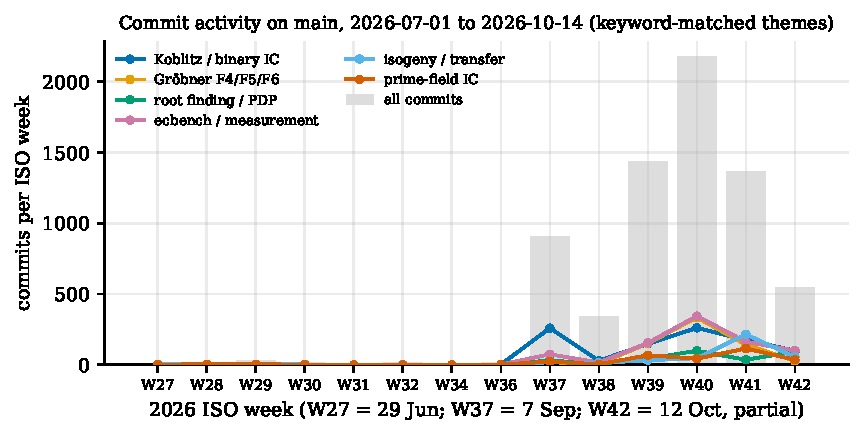
\includegraphics[width=\linewidth]{figures/fig-timeline.pdf}
\caption[]{Commits per ISO week on \texttt{main}, 1 July--14 October 2026
(6{,}882 commits; week 42 partial). Lines: commits whose subject matches
each theme's keywords. Source: \texttt{git log} at the paper's base commit;
values in \art{figures/data.json}.}
\label{fig:timeline}
\end{figure}

\paragraph{Prelude: July and August.} The prime-field \emph{ecdlp
autolab} ran numbered threads on curve structure---universal order-2
Frobenius forms, the CM-73 family $\{19,37,79,109\}$, sextic-twist pairs
that are Howe-glueable (5 of 15)---and its draft ``An Empirical
Resistance Map for Prime-Field ECDLP''
(\art{research/ecdlp_autolab/PAPER_DRAFT.md}). Those threads found
structure but no solver advantage, which is what turned the programme
towards index calculus, where structure is supposed to pay.

\paragraph{Phase 1, 6--14 September: Koblitz index calculus from
scratch.} The ECC2K-130 rho client and an audit of a public
index-calculus benchmark's SAT/UNSAT labels (6 Sept) were followed by
Frobenius-invariant factor bases with a matrix-F4 Semaev oracle, an
XOR-native SAT oracle after Trimoska et al.\ (7 Sept), and a $\sim50\times$
faster Semaev solve the same day. On 8 September a scaling experiment
showed the SAT route does not scale and that the refutation frontier
belongs to F4; pairs-and-solve replaced triple enumeration for
$\Sem4$. The boundary ledger was codified on 10 September, together with
a meet-in-the-middle oracle, incremental modular linear algebra and a
CADO-style split into factor-base logs then descent. A burst of more than
100 numbered pipeline stages (12--13 Sept: PCLMUL field products, fused
pair collection, scalar-blind targets, rank-aware scans) took the
multi-target $n=53$ pipeline to a 1{,}024-target process-wall crossover
against batched rho. On 13--14 September six pre-registered ECC2K-130
decomposition experiments ran (``exists, admissible, not findable''; no
falsifier fired), and the repository began to require frozen benchmarks
and full-pipeline evidence for any ECDLP speed claim.

\paragraph{Phase 2, 15 September--1 October: engines and the compact
orbit.} Inherited F4 (22 Sept) became the default algebraic oracle; a fast
binary-field hot path, Itoh--Tsujii inversion and a parallel radix-sorted
pair-table build landed (23--24 Sept); a long Boolean F4/F5 kernel series
(AVX2/AVX-512 unpackers, compact columns, pivot orders; 26 Sept--3 Oct)
ran in parallel. The compact signed-Frobenius orbit producer beat batched rho on
multi-target $n=61$ batches (25--26 Sept), and from 2 October carried the
one-target online ladder to $n=71$ and (6 Oct) $n=73$ on 128-bit words,
after $n=63$ was closed as non-viable. A fixed-policy
cold comparison on orbit-disjoint public points (1 Oct) was a measured
no-go.

\paragraph{Phase 3, 2--10 October: one harness, and the audit it
forced.} \emph{ecbench} landed on 2 October. F6-IC and a 23-study $n=83$
campaign (4--6 Oct), the registered $m=3$ refutation-degree law (5--11
Oct), the ECC2K-130 feasibility extrapolation (5 Oct), the accounting
correction plan, conductor-gap and novel-direction notes (7 Oct), and the
transfer-aware, isogeny-fibre and Gr\"obner-engine audits (10 Oct)
followed.

\paragraph{Phase 4, 11--14 October: literature, root finding,
consolidation.} The lit2026 programme (11 Oct) turned a literature search
into twelve workstreams. A supplied manuscript on root-finding
decomposition was frozen, audited and re-measured in ecbench (12 Oct), and
the identity it rests on was generalised across PDP oracles, a CUDA
kernel, Kummer towers, Koblitz engines and dense root indices (12--14
Oct). The admitted $n=61$ online panel ran on two hosts (12 Oct). Gaudry's
$k=4$ solve was made generic and given the $D_4$ symmetry; the frontier
synthesis and its replay audit closed the period (13 Oct); the last
root-finding loops priced F4's word XORs and ran out of levers against rho
(14 Oct).

\paragraph{Phase 5, 14--15 October: measured against the baseline.} Two
improvement rounds and a next-steps campaign paired each change against
the index-calculus incumbent under frozen protocols
(\S\ref{sec:ladder}): genus-3 index calculus after the cubic GHS transfer,
the $k=4$ ladder and its four-unknown solve, production free relations and
oracle row harvesting on Koblitz curves, and a CADO-NFS-derived filter for
the linear algebra. An equal-advice audit retired the online win (14 Oct).
The owner then fixed the success criterion as iterative improvement over
that baseline, with the gap to rho as distance remaining (15 Oct), and the
priced frontier campaign of \S\ref{sec:campaign} ran the same day.
